\documentclass[a4paper,11pt]{article}
\usepackage{amsmath,amsthm,amsfonts,amssymb,amscd,amstext,vmargin,graphics,graphicx,tabularx,multicol} \usepackage[french]{babel}
\usepackage[utf8]{inputenc}  
\usepackage[T1]{fontenc} 
\usepackage[T1]{fontenc}
\usepackage{amsmath,amssymb}
\usepackage{pstricks-add,tikz,tkz-tab,variations}
\usepackage[autolanguage,np]{numprint} 
\usepackage{color}
\usepackage{ulem}

\setmarginsrb{1.5cm}{0.5cm}{1cm}{0.5cm}{0cm}{0cm}{0cm}{0cm} %Gauche, haut, droite, haut
\newcounter{numexo}
\newcommand{\exo}[1]{\stepcounter{numexo}\noindent{\bf Exercice~\thenumexo} : \marginpar{\hfill /#1}}
\reversemarginpar


\newcounter{enumtabi}
\newcounter{enumtaba}
\newcommand{\q}{\stepcounter{enumtabi} \theenumtabi.  }
\newcommand{\qa}{\stepcounter{enumtaba} (\alph{enumtaba}) }
\newcommand{\initq}{\setcounter{enumtabi}{0}}
\newcommand{\initqa}{\setcounter{enumtaba}{0}}

\newcommand{\be}{\begin{enumerate}}
\newcommand{\ee}{\end{enumerate}}
\newcommand{\bi}{\begin{itemize}}
\newcommand{\ei}{\end{itemize}}
\newcommand{\bp}{\begin{pspicture*}}
\newcommand{\ep}{\end{pspicture*}}
\newcommand{\bt}{\begin{tabular}}
\newcommand{\et}{\end{tabular}}
\renewcommand{\tabularxcolumn}[1]{>{\centering}m{#1}} %(colonne m{} centrée, au lieu de p par défault) 
\newcommand{\tnl}{\tabularnewline}

\newcommand{\trait}{\noindent \rule{\linewidth}{0.2mm}}
\newcommand{\hs}[1]{\hspace{#1}}
\newcommand{\vs}[1]{\vspace{#1}}

\newcommand{\N}{\mathbb{N}}
\newcommand{\Z}{\mathbb{Z}}
\newcommand{\R}{\mathbb{R}}
\newcommand{\C}{\mathbb{C}}
\newcommand{\Dcal}{\mathcal{D}}
\newcommand{\Ccal}{\mathcal{C}}
\newcommand{\mc}{\mathcal}

\newcommand{\vect}[1]{\overrightarrow{#1}}
\newcommand{\ds}{\displaystyle}
\newcommand{\eq}{\quad \Leftrightarrow \quad}
\newcommand{\vecti}{\vec{\imath}}
\newcommand{\vectj}{\vec{\jmath}}
\newcommand{\Oij}{(O;\vec{\imath}, \vec{\jmath})}
\newcommand{\OIJ}{(O;I,J)}

\newcommand{\bmul}[1]{\begin{multicols}{#1}}
\newcommand{\emul}{\end{multicols}}


\newcommand{\reponse}[1][1]{%
\multido{}{#1}{\makebox[\linewidth]{\rule[0pt]{0pt}{20pt}\dotfill}
}}

\newcommand{\titre}[5] 
% #1: titre #2: haut gauche #3: bas gauche #4: haut droite #5: bas droite
{
\noindent #2 \hfill #4 \\
#3 \hfill #5

\vspace{-1.6cm}

\begin{center}\rule{6cm}{0.5mm}\end{center}
\vspace{0.2cm}
\begin{center}{\large{\textbf{#1}}}\end{center}
\begin{center}\rule{6cm}{0.5mm}\end{center}
}



\begin{document}
\pagestyle{empty}
\titre{Contrôle 2 : Transformations}{Nom}{Prénom}{Date}{Classe}

\begin{flushleft}
\begin{tabular}{|m{9.5cm}|m{1.25cm}|m{1.25cm}|m{1.25cm}|m{1.25cm}|m{1.25cm}|}
\hline 
\textbf{Compétences} & \begin{center}
\textbf{N.E.}
\end{center} & \begin{center}
\textbf{M.I.}
\end{center} & \begin{center}
\textbf{M.F.}
\end{center}  & \begin{center}
\textbf{M.S.}
\end{center} & \begin{center}
\textbf{T.B.M.}
\end{center} \\ 
\hline 
Je dois comprendre l'effet d'une symétrie (axiale et centrale) sur une  figure et savoir construire l'image d'une figure par une des symétries &  &  & & &\\
\hline 
Je dois comprendre l'effet d'une translation sur une  figure et savoir construire l'image d'une  figure par une translation&  &  & & &\\
\hline
Je dois comprendre l'effet d'une rotation sur une  figure et savoir construire l'image d'une figure par une rotation &  &  & & &\\ 
\hline


\end{tabular} 
\end{flushleft}

\textit{N.E = Non évalué ; M.I. = Maîtrise insuffisante ; M.F. = Maîtrise fragile ; M.S. = Maîtrise satisfaisante ; T.B.M. = Très bonne maîtrise}\\

\vspace*{0.3cm}



\exo{3} Un pavage du rectangle IJKL ci-dessous est réalisé à l'aide de 24 pièces superposables. Ces pièces sont numérotées de 1 à 24.\\

Répondre aux questions \textbf{sur votre copie simple} :

\bmul{2}
\includegraphics[scale=1]{exobrevet2.eps} 

\columnbreak



\qa Quelle est l'image de la pièce 5 par la symétrie d'axe (CD) ?\\

\qa Quelle est l'image de la pièce 3 par la symétrie de centre B ?\\

\qa Dans la translation qui transforme C en B, quelle est l'image de la pièce 3 ?\\

\qa Dans la rotation de centre A et d'angle 90 degré, dans le sens des aiguilles d'une montre, quelle est l'image de la pièce 6?\\


\emul





\exo{2} Construire le symétrique F2 de la figure F1 par rapport à la droite (d) puis construire le symétrique F3 de la figure F1 par rapport au point S.


\begin{center}
\includegraphics[scale=0.8]{exosymetries1.eps} 
\end{center}

\newpage



\vspace*{0.5cm}
\exo{4}\\



\textbf{Sur le sujet,} \\

\initqa
\noindent \qa construire l'image du nombre 2 000 par la rotation de  centre  O,  d'angle  90\degre,  dans  le sens inverse des aiguilles d'une montre;\\
\qa construire l'image du nombre 2 000 par la translation qui transforme le point A en C.\\

\vspace*{0.5cm}

\includegraphics[scale=1=0.8]{exobrevet.eps} \\
\vspace*{1.5cm}


\exo{4} \textbf{Sur le sujet}, tracer A'B'C'D'E', l'image du polygone ABCDE par la translation qui transforme D en D'.\\
 

\includegraphics[scale=0.9]{exotranf4.eps} \\

\newpage
\vspace*{0.5cm}

\exo{4}\\

 \textbf{Sur le sujet}, construire l'image du carré ABCD par la rotation   de   centre   D,   d'angle   45\degre   dans   le   sens inverse des aiguilles d'une montre.\\

\vspace*{1.5cm}


\begin{center}
\includegraphics[scale=0.9]{rotation.eps} \\
\end{center}

\vspace*{2.5cm}



\vspace*{1.5cm}

\exo{3}

\begin{center}
\includegraphics[scale=1]{exotranf6.eps} 
\end{center}

\initq 
Le trapèze KLMN est l'image du trapèze ABCD par une translation.\\
\q  Cette translation transforme quel point en quel point ? Caractériser cette translation par une flèche sur le sujet.\\
\q Déterminer la mesure de l'angle $\widehat{KLM}$. Justifier.\\
\q Déterminer la distance LM. Justifier.\\

$\rightarrow$ \textbf{QUESTION BONUS} : Calculer l'aire du trapèze KLMN.\\

\end{document}
